\documentclass[a4paper,11pt]{article}
\usepackage{tikz}
\usetikzlibrary{shapes}
\usetikzlibrary{plotmarks}
\usepackage{tikz-3dplot}

\begin{document}

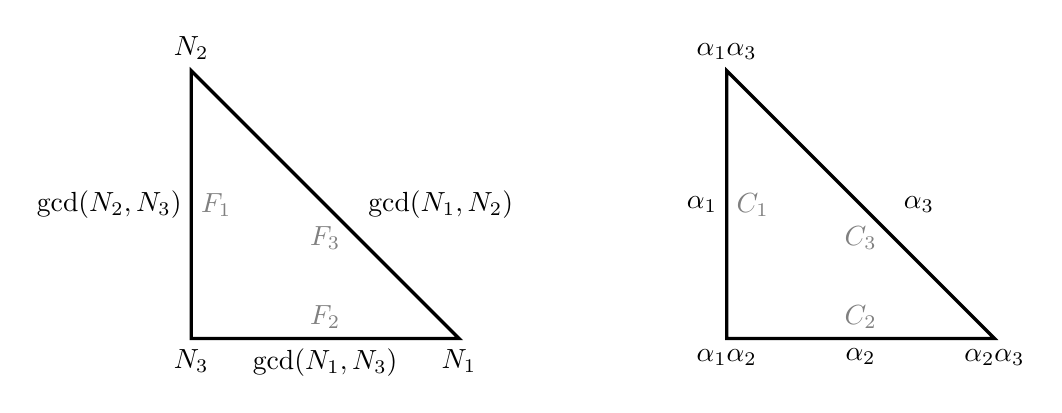
\begin{tikzpicture}[scale=.85]
    \draw[line width=1.2pt] (0,0) node[below]{$N_3$}--(4,0) node[below]{$N_1$}--(0,4) node[above]{$N_2$}--cycle;
    \node at (2,0) [below,align=center]{$\gcd(N_1,N_3)$};
    \node at (2,0) [above,gray]{$F_2$};
    \node at (0,2) [left,align=center]{$\gcd(N_2,N_3)$};
    \node at (0,2) [right,gray]{$F_1$};
    \node at (2.5,2) [right,align=center]{$\gcd(N_1,N_2)$};
    \node at (2,1.5) [gray]{$F_3$};
    \begin{scope}[shift={(8,0)}]
        \draw[line width=1.2pt] (0,0) node[below]{$\alpha_1\alpha_2$}--(4,0) node[below]{$\alpha_2\alpha_3$}--(0,4) node[above]{$\alpha_1\alpha_3$}--cycle;
        \node at (2,0) [below,align=center]{$\alpha_2$};
        \node at (2,0) [above,gray]{$C_2$};
        \node at (0,2) [left,align=center]{$\alpha_1$};
        \node at (0,2) [right,gray]{$C_1$};
        \node at (2.5,2) [right,align=center]{$\alpha_3$};
        \node at (2,1.5) [gray]{$C_3$};
    \end{scope}
\end{tikzpicture}

\end{document}